%\vspace{-1em}
\section{Analysis: Why does CRL Struggle with Interactions in Manipulation?}
%\vspace{-1em}
\label{sec: analysis}
%The success of CRL depends on whether the inner-product energy $E_{\phi,\psi}(s,a,g)=\phi(s,a)^\top\psi(g)$ can faithfully represent the future-density ratio $E^\star(s,a,g)
%    =
%    \log \rho^\pi(g\mid s,a)
%    -
%    \log \bar{\rho}^{\pi}_{\mathcal{B}}(g)$.
The success of CRL depends on whether the inner-product energy $E_{\phi,\psi}(s,a,g)$ can faithfully represent the future-density ratio $E^\star(s,a,g)$.
This motivates our analysis: what class of future distributions is naturally represented by the inner-product CRL energy function, and when does this representation become insufficient? Building on the Gaussian idealization behind temporal interpolation in CRL~\citep{eysenbach2024inference}, we first revisit why contrastive representations are well-suited to smooth, single-mode dynamics, and then show why this structure breaks down in manipulation, where interactions induce latent mode changes and piecewise nonlinear future distributions.
%\vspace{-1em}
\subsection{CRL as a Linear-Gaussian Temporal Model}
\label{subsec:crl-gaussian-view}
%\vspace{-1em}
We begin from the Gaussian idealization of temporal contrastive representations. \citet{eysenbach2024inference} show that CRL induces a simple linear-Gaussian model of discounted future occupancy in representation space. In particular, when the marginal representation distribution is approximately isotropic Gaussian and the contrastive density ratio is represented by a quadratic score, the conditional future representation admits a Gaussian form,
\begin{equation*}
    p(\psi_{t+n}\mid \psi_t)
    =
    \mathcal N(\mu_n(\psi_t),\Sigma_n).
\end{equation*}
Naturally, for a single-mode MDP, the temporal mean can be parameterized by a single linear operator $A$, yielding
\begin{equation}
    \mu_n(\psi_t) = A^n\psi_t,
    \qquad
    p(\psi_{t+n}\mid \psi_t)
    =
    \mathcal N(A^n\psi_t,\Sigma_n).
\end{equation}
All temporal structure is generated by powers of the same operator $A$. The geometrically sampled future states used by CRL provide dense supervision for estimating this temporal operator across different horizons, which explains the strength of CRL in navigation and locomotion domains. Essentially, CRL can be understood as learning a smooth Gaussian-like geometry for future reachability.

% This explains the empirical strength of CRL in navigation and locomotion domains~\citep{eysenbach2022contrastive}. When the action affects the same state variables that define the future goal, and the resulting reachability structure is organized by a single smooth temporal mode -- an inner-product CRL critic can learn a representation in which temporal interpolation and planning are well behaved. In this sense, CRL can be understood as learning a smooth Gaussian-like geometry for future reachability.
%\vspace{-0.8em}
\subsection{Manipulation Induces Mode-Conditioned Gaussian Futures}
%\vspace{-0.8em}
\label{subsec:mode-conditioned-gaussian}
However, the single-operator Gaussian view becomes insufficient in manipulation. Unlike locomotion domains, where the action persistently affects the same state variable used as the future goal, manipulation often separates the actuated factor from the target factor. Let the state be factored as $s_t=(u_t,y_t)$,
where $u_t$ denotes the actuated factor, such as the robot end-effector or paddle, and $y_t$ denotes the target factor, such as an object or puck, and the state-action anchor is $x_t=(u_t,y_t,a_t)$.

In the average case, actions do not always affect the target factor. Instead, their effects are activated only through interaction events. We represent this using an interaction indicator $\omega_t=m(x_t)\in\{0,1\}$,
where $\omega_t=0$ denotes \textit{passive} target dynamics and $\omega_t=1$ denotes an interaction mode. The target dynamics can then be written as a piecewise transition:
\begin{equation}
y_{t+1}
=
\begin{cases}
f_0(y_t), & \omega_t=0,\\
f_1(u_t,y_t,a_t), & \omega_t=1.
\end{cases}
\label{eq:piecewise-target-dynamics}
\end{equation}
In the passive mode, the target dynamics are without direct dependence on the robot action; in the interaction mode, the target dynamics depend on the actuated factor and action.

Applying the Gaussian temporal view mode-wise yields a different representation-level future model for each mode. Let \(\psi_t=\psi(y_t)\) be the target-factor representation. In the \textit{passive mode}, the future representation can be approximated by a target-only temporal operator, $\psi_{t+1}=A_0\psi_t+\epsilon_t$.
In the \textit{interaction mode}, however, the target update includes an additional displacement induced by the actuated factor and action:
    $\psi_{t+1}
    =
    A_1\psi_t + b_t + \epsilon_t$,
    $b_t = B(u_t,y_t,a_t)$.

Combining the two cases, manipulation induces a switched affine Gaussian model:
\begin{equation}
    \psi_{t+1}
    =
    A_{\omega_t}\psi_t
    +
    \omega_t b_t
    +
    \epsilon_t,
    \qquad
    \epsilon_t\sim\mathcal N(0,\Sigma_{\omega_t}).
    \label{eq:switched-affine-gaussian}
\end{equation}
This indicates the \textit{structural mismatch} between manipulation and the single-mode CRL geometry. Interactions change the active mode of the representation dynamics and introduce an interaction residual $b_t$ that depends on the robot-object relation and action. As a result, the future representation is no longer governed by powers of a single operator $A$, but by a sequence of mode-dependent operators and interaction residuals. An illustration is in Fig.~\ref{fig:theory_illustration}.
\begin{figure}[h]
    \vspace{-8pt}   
    \centering
    \small
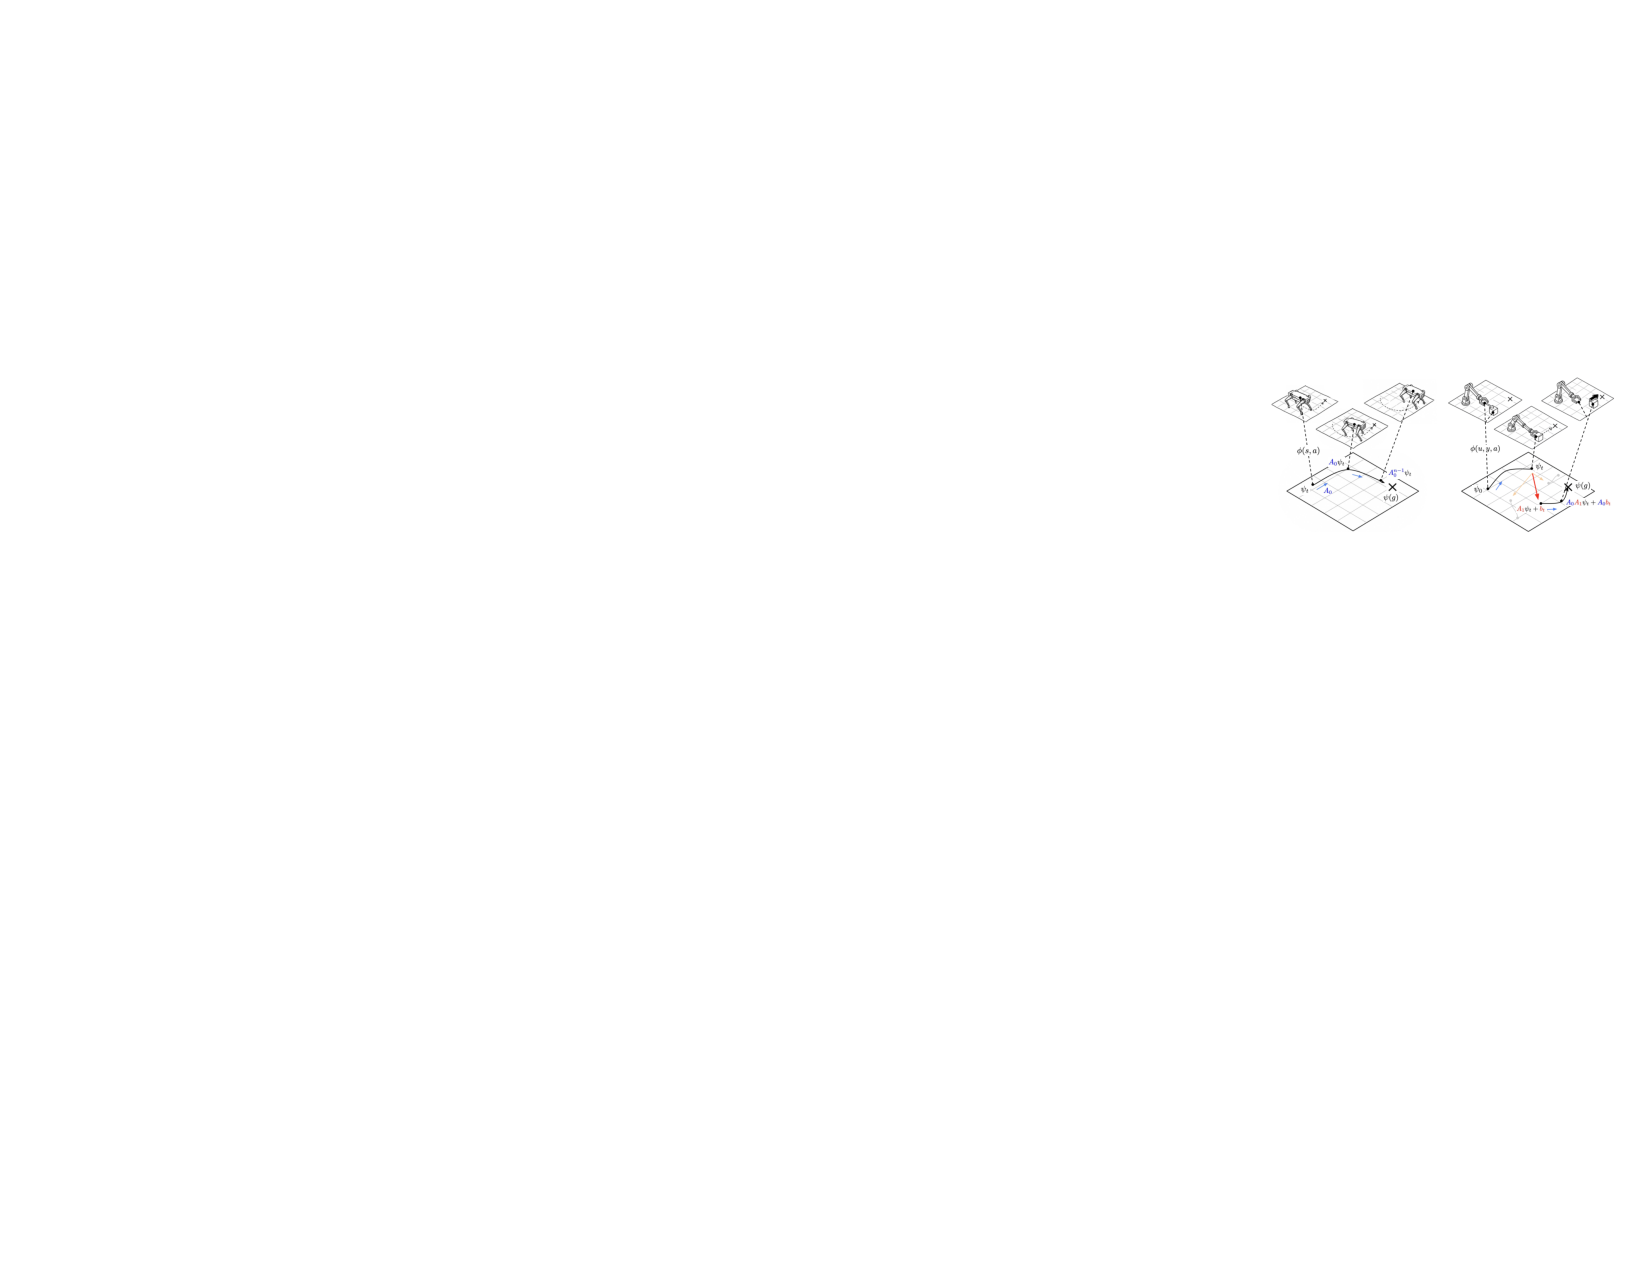
\includegraphics[width=1.0\linewidth]{figure/theory-illustration.pdf}
    \caption{\textbf{Interaction-induced mode changes break the single-operator CRL geometry}. In smooth locomotion domains, future representations can often be organized by repeatedly applying a single temporal operator, producing a coherent trajectory toward the goal. In manipulation, interactions such as contact or object transfer switch the active dynamics and introduce residual displacements that depend on the actuated factor and action. Hence, the future distribution becomes piecewise and branching, making standard CRL smoothing over critical interaction transitions.}
    \label{fig:theory_illustration}
    \vspace{-.5cm}
\end{figure}
%\textcolor{red}{An illustration in Appendix xxx}
%\vspace{-0.8em}
\subsection{Two Challenges for CRL in Interaction-Rich Manipulation}
%\vspace{-0.8em}
The mode-conditioned Gaussian reveals two distinct challenges for applying CRL to manipulation. 

\textcolor{darkred}{\textbf{Sampling Challenge}}: Standard CRL learns from endpoint pairs $(x_t,y_f)$, where $y_f$ is sampled as a discounted future. However, the interaction event that changes the target dynamics may occur only at a sparse and latent time $\tau_t$. If the sampled future lies before the interaction, the tuple only observes passive target evolution and provides no direct supervision for the interaction-induced shift. If the sampled future lies far after the interaction, the effect of the interaction is propagated through subsequent passive dynamics, which can attenuate or mix the signal. As a result, ordinary contrastive sampling can be dominated by smooth pre-interaction or post-interaction transitions, while the critical bridge transition that changes the dynamic mode remains underrepresented. 

\textcolor{darkred}{\textbf{Error Propagation}}: Even when an interaction-crossing future is sampled, the interaction information may be observed only after it has propagated through subsequent target dynamics.
This makes the learned energy fragile around contact.
We formalize this issue in the one-reset case, where the target first evolves passively, then experiences one interaction, and then evolves passively again.

\begin{proposition}[Error Propagation]
\label{prop:endpoint-energy-error} Let $e$ denote the local interaction-bridge estimation error, and let $k$ denote the number of passive steps after the interaction. 
In the one-reset case, the endpoint energy error scales as
\begin{equation}
    \sup|\widehat{E}_k - E_k|
    \propto
    \|A_0^k\|
    \|e\|
    +
    \frac{1}{2}
    \|A_0^k\|^2
    \|e\|^2 .
    \label{eq:energy-error-bound-main}
\end{equation}
\end{proposition}
Proposition~\ref{prop:endpoint-energy-error} shows that the endpoint energy error depends on two factors: the local bridge estimation error $\|e\|$ and the post-interaction propagation factor $\|A_0^k\|$. 
In manipulation, after contact the target often evolves passively and cannot be corrected by the robot.
Therefore, an inaccurate interaction shift is carried forward by the passive dynamics, producing fragile energy estimates and inaccurate actor gradients near the interaction.
In tasks with repeated or branched interactions, such as pick-place, this issue becomes more severe because the future distribution becomes a mixture over multiple interaction times and interaction residuals. More detailed theorems, analysis, and the full proof can be found in Appendix~\ref{app:theory}. 
